

Developers use logging statements to yield useful information about the state of an application during its execution. This information is collected in files (logs) and contains details  which would otherwise be difficult to collect, such as the value of variables. Logs are used during various development activities such as fixing bugs~\cite{ConsoleLogs,JGLouMining,QFuanomaly}, analyzing load tests~\cite{Automatic}, monitoring performance~\cite{Yuan} and transferring knowledge~\cite{IanWCRE}.
Logging statements make use of logging libraries or more archaic methods such as \textsl{print} statements. Every logging statement contains a textual part, which provides information about the context, a variable part providing context information about the event and a log level, which shows the verbosity of the logging statement. An example of a logging statement is in Figure~\ref{fig:logexample}.
% shown below where info is the logging level, \textsl{Testing Connection to Host Id} is the context information and \textsl{host}, which is the variable part, provides information about the logging context.
%\hypobox{LOG.info(``Testing Connection to Host Id:" + host);}

\begin{figure}[thb]
	\centering
	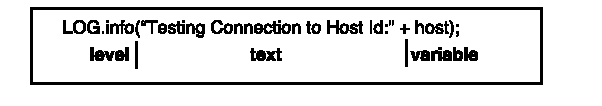
\includegraphics[width=1\columnwidth]{logexample}
	\caption{Example of a logging statement}
	\label{fig:logexample}
\end{figure}




The rich knowledge in logs has lead to the development of many enterprise log processing tools such as \textsl{Splunk}~\cite{carasso2012exploring}, \textsl{Xpolog}~\cite{xpolog}, \textsl{Logstash}~\cite{xu2013detecting} and research tools such as Salsa~\cite{TanSalsa}, log-enhancer~\cite{Yuan} and Chukwa~\cite{chukwa} which are designed to analyze logs as well as improve logging statements. However, when logging statements are changed, the associated log processing tools may also need to be updated. For example, Figure~\ref{fig:ExampleOfLogChange_LPA} demonstrates a case in which a developer removes the elapsed time for an event. Removing information from a logging statement can affect log processing tools that rely on the removed information in order to monitor the health of the application. Prior research shows that 60\% of the logging statements that generate output during system execution are changed and affect the log processing tools that heavily depend on the logs that are generated by these logging statements~\cite{IanWCRE}.

Knowing whether a logging statement is likely to change in the future is helpful to reduce the effort required to maintain log processing tools. If a developer of a log processing tool knows that a logging statement is likely to change, the developer can opt not to depend on the parts of the log that are generated by this logging statement. Instead, the developer can let the log processing tool depend on output generated by logging statements that are likely to remain unchanged. Depending on logging statements that remain unchanged will reduce the maintenance effort required for keeping the log processing tool consistent with ever-changing logs. 

%As changes to logging statements can affect the log processing tools depending on them, it is necessary to identify the cause for these logging statement changes. 

To decide whether a logging statement will change in the future, we must understand which factors play an important role during such a change. The following factors can influence whether a logging statement will change:
\begin{enumerate}
\item The contents of the logging statement
\item The location of the logging statement
\item The developer who added the logging statement to the source code
\end{enumerate}
In this paper, we examine which of these factors can help to decide whether a logging statement will change. First, we present a preliminary study which was done to get a better understanding of the stability of logging statements in four open source projects. In this preliminary study, we find that 25\%-45\% of the logging statements are changed at least once during their lifespan in the studied applications, which shows that developers of log processing tools have to carefully select the logging statements they will depend on. 

Second, we extract the factors that are important for explaining the stability of a logging statement using a random forest classifier. This classifier uses metrics that describe the three factors mentioned above to decide the likelihood of a log change.
The most important observations in this paper are:

%We identify three main factors which can cause changes in logging statements namely: 1) who introduces and changes logs, 2) where the logging statement are placed, and 3) what is content of the logged statement.  


% These log changes can affect the log processing tools which heavily depend on them and maintenance cost will be high~\cite{IanWCRE}. 
\begin{figure}[tb]
	\centering
	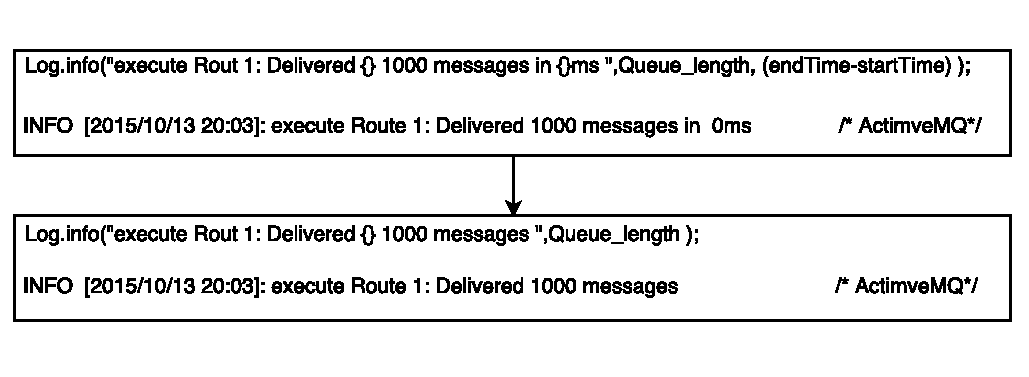
\includegraphics[width=1\columnwidth]{ExampleOfLogChange_LPA}
	\caption{Modification of a logging statement}
	\label{fig:ExampleOfLogChange_LPA}
\end{figure}

\begin{figure*}
	\centering
	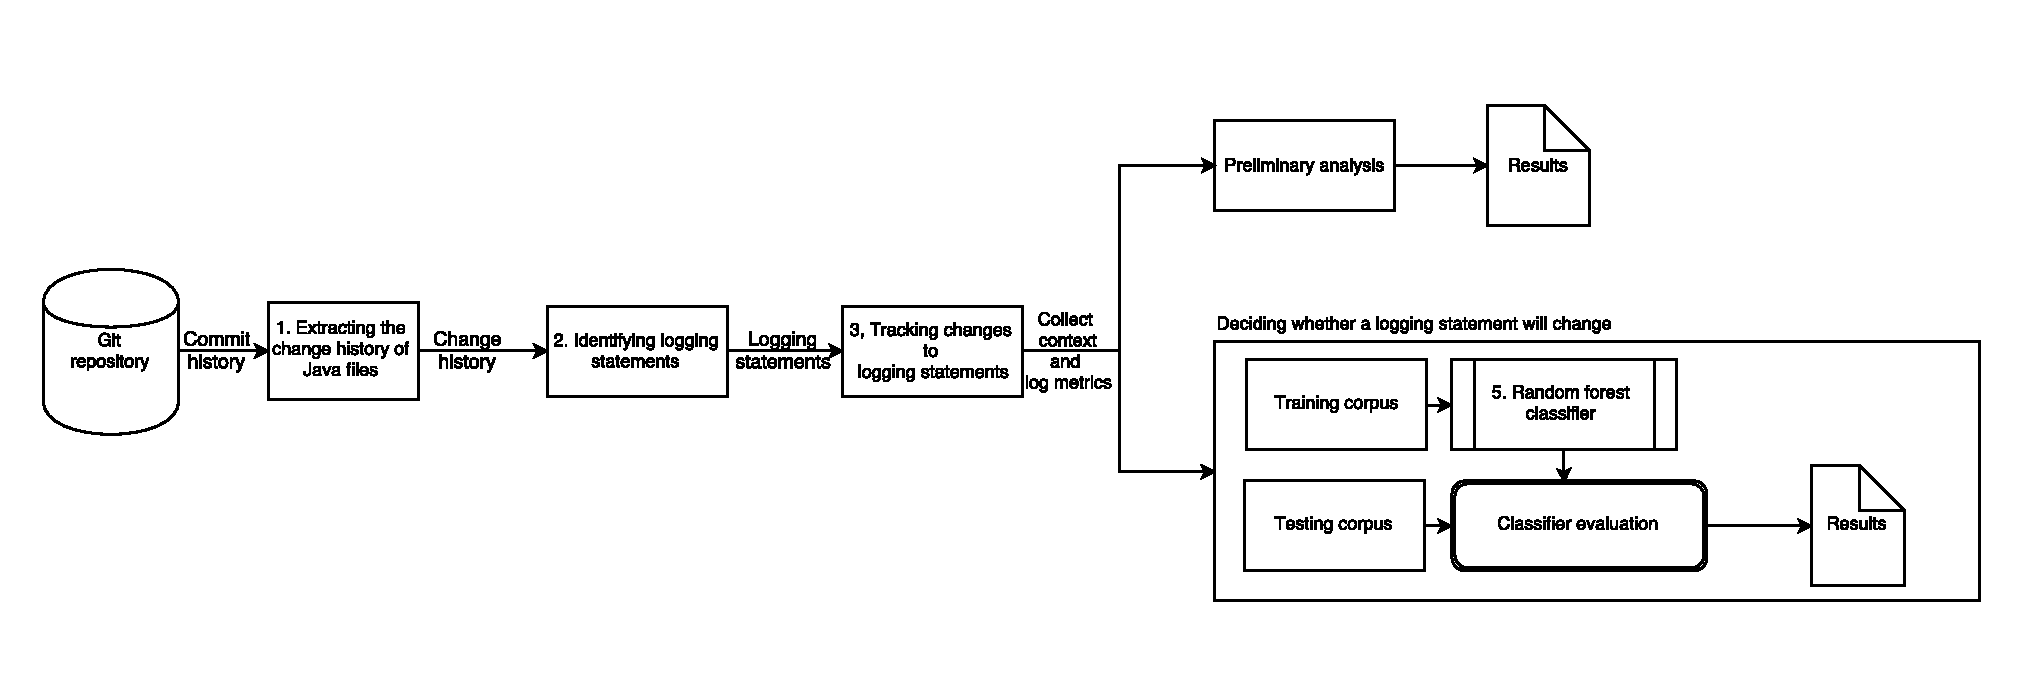
\includegraphics[width=1\textwidth,
	height=.4\textwidth]{LogGenalogyMethdology}
	\caption{Overview of the data extraction and empirical study approach}
	\label{fig:LGmethod}
\end{figure*}


%To identify the influence of these factors, in this paper we first study how much logging statements are changed across multiple releases in the four software applications. We find that 35\%-50\% of the logging statements are changed at least once during their lifespan in the studied applications. We also find that a single log changes between 0 to 10 times within its lifetime and can be changed by more than one developer. These results suggest that log processing tools have to be constantly monitored at every release to prevent breakage by the changes to logging statements. 

%To identify which factors the stability of logging statements and model which logs will change in the future, we build a random forest classifier using context and log metrics. The most important observations in this paper are:
\begin{enumerate}
	\item We can decide which logging statements will be changed in the future using a \emph{random forest} classifier with a precision of 83\%-91\% and recall of 65\%-85\%.
%	Our \textsl{random forest} achieves an precision of 89\%-91\% and recall of 71\%-83\%, when predicting which logs will be changed.


	\item Logging statements added  by highly experienced developers and very new developers are less likely to be changed. We find that in three of the studied applications the top three developers add more than 60\% of the logging statements and 70\% of their logging statement remain untouched. 
	
	
	\item Logging statements added by developers who have less ownership on the file have higher likelihood of being changed. We find that
	27\%-67\% of all log changes, are done on logging statement added by developers who own less than 20\% of the file.
	
%	logging statements added by developers who own less than 20\% of the file are, 1.2-1.6 times more likely to be changed later.
%	 27\%-67\% of all logging statement changes, are done on logging statement added by developers who own less than 20\% of the file. 
	
	
%	\item FIXME Logging statements changed by developers who have less ownership in that file are 0.4-1.4 times more likely to be changed again than logs changed by owners of the file in three of the applications.
%	\item FIXME Developer experience is negatively correlated to log stability in the studied applications, suggesting that logs added by more experienced developers are more stable. This findings suggest that knowledge of the code in a file is important when considering the stability of a logging statement. As a result, maintainers of log processing tools can take special care when importing log statements written by developers who have less experience or with no ownership of the file in which the statement was added.
	\item Large files (i.e., SLOC is 2x-3x the median) with lower log density, are more likely to have logging statement changes than well logged files.

%	\item  Change metrics such as SLOC, number of variables logged and number of variables declared are strong predictors of log stability within the studied applications. 

\end{enumerate}

From the above findings, maintainers of log processing tools can be more selective when importing logging statements to be used by their tools and decrease the maintenance effort.

%should be careful when importing log statements written in larger file with less number of logs. 


%These log processing tools are used to generate information for capacity planning of large-scale systems~\cite{hassan2008industrial,nagappan2009efficiently}, to monitor system health~\cite{bitincka2010optimizing} or to detect abnormal system behavior~\cite{JiangICSM2008}. These tools rely heavily on the log messages themselves and require continuous maintenance when the format or content of logs are changed.

% and use the data to answer the following research questions.

%\textbf{RQ1:} \textbf{How much do logs change over time and why do the changes occur?}
%
%Based on our quantitative analysis of the studied systems we identify three categories of change frequency in logs. If a log is changed more than four times we categorize it as \textsl{`Frequently Changed'}, if it has one to three changes, it is categorized as \textsl{`Changed'} and if there are no changes made we categorize it as \textsl{`Never Changed'}. We find that in our studied systems, 20-80\% of the logs are changed at least once throughout their lifespan.


%\textbf{RQ2:} \textbf{Can metrics from code, log and developer dimension help in explaining the stability of logs?}

%We collect the product and change metrics from three dimensions namely code, log and developer information. Our \textsl{random forest} achieves an accuracy of 89\%-91\% and recall of 71\%-91\%, when predicting which logs have higher likelihood of getting changed. We also identify significant metrics from each of the three dimensions, that affect the stability of logs. We find  developer experience, source lines of code, file ownership, log density in the file are strong predictors in classifying if a log will change in the future. 
 
 
% Our results show that product and process metrics obtained from code, log and developer information can help in identifying unstable logs in our studied systems. This can help in reducing the effort needed in the maintenance of log processing applications, as system maintainers can flag the logs that have the potential of being changed in subsequent releases and track them. 
 
The remainder of this paper is organized as follows. Section~\ref{analysis} presents the preliminary analysis to motivate our study. Section~\ref{prediction} describes the random forest classifier and the analysis results. Section~\ref{related} describes the prior research that is related to our work. Section~\ref{threats} discusses the threats to validity. Finally, Section~\ref{conc} concludes the paper.
 
 
% However, as these tools are not scalable for all companies and systems, companies prefer in house development or customization of these tools for their specific purposes. 